\vssub
\subsubsection{~Triangular unstructured grids} \label{sub:num_space_tri}
\conthead{WWM-II}{A. Roland, F. Ardhuin, M. Dutour-Sikiri\'c}

\noindent Triangle-based grids can be used in \ws\ by using numerical schemes
based on contour residual distribution (RD) \citep[see][for a
review]{rep:Roland2008}.  These schemes have been 1st time implemented in the 
WWM-II and have been used efficiently in WWM-II as well as in WWIII \citep[e.g.][]{art:Aea09,Magne2010}.
This option is activated by setting the grid string
to `{\code UNST}' in {\file ww3\_grid.inp}.  Four schemes have been
implemented, and the choice of one or the other is done with the {\code UG}
namelist.  These are the CRD-N-scheme (1st order), the CRD-PSI-scheme 
(better than 1st order, 2nd order on triangular strucutured grids), 
the CRD-FCT-scheme (2nd order space-time, and
the implicit N-scheme. The default is the most efficient but 1st order 
diffusive explicit N-scheme. An implicit variant of the RD-Schemes using the method of lines
and the N-Scheme for the space discretization was implemented in the SWAN model by \citet{Zijlema2010267}.

In practice the grid can be easily generated, using the PolyMesh interface
(software developed by Aron Roland), from a shoreline polygons database
\citep[e.g.][]{art:WS96} and a list of depth soundings, regular or irregular.

Regarding the method: the evolution of the spectrum at the nodes, where it is
evaluated, is based on the redistribution over the nodes of the flux
convergence into the median dual cells associated with the nodes (see figure
\ref{fig:triangles}).  For any spectral component, the advection equation
(\ref{eq:step_xy_prop}) is solved on the median dual cells: the incoming flux
into a cell gives the rate of change of the wave action at the corresponding
node. The various schemes implemented have different discretizations for the
estimation of this flux. The schemes have been presented in \citep[see][for a
review]{rep:Roland2008} and \citet{RolandECMWF}.

The equivalent of the CFL condition in the stable schemes is the ratio of the
dual cell area divided by the product of the time step and all positive flux
into the dual cell. Because the spectral levels are imposed on the boundary
for the positive fluxes, the boundary nodes are excluded from this CFL
calculation and the incoming energy is set to zero, whereas the outgoing energy 
is fully absorbed. 

The boundary condition at the shoreline depends on the wave direction
relative to the shoreline orientation. This particular treatment is enforced
using the `{\code IOBPD}' array which is updated whenever the grid points
status map `{\code MAPSTA}' changes. The grid geometry is also used to define
local gradients of the water depth and currents. All other operations, such as
interpolation of the forcing on the grid and interpolation from the grid onto
output locations, is performed using linear interpolation in triangles.

All the triangle geometry operations assume a locally flat Earth. Depth and
current gradients on the grid are estimated at the nodes by weighting with
their angle the gradients over each triangle connected to the node.

\begin{figure} \begin{center}
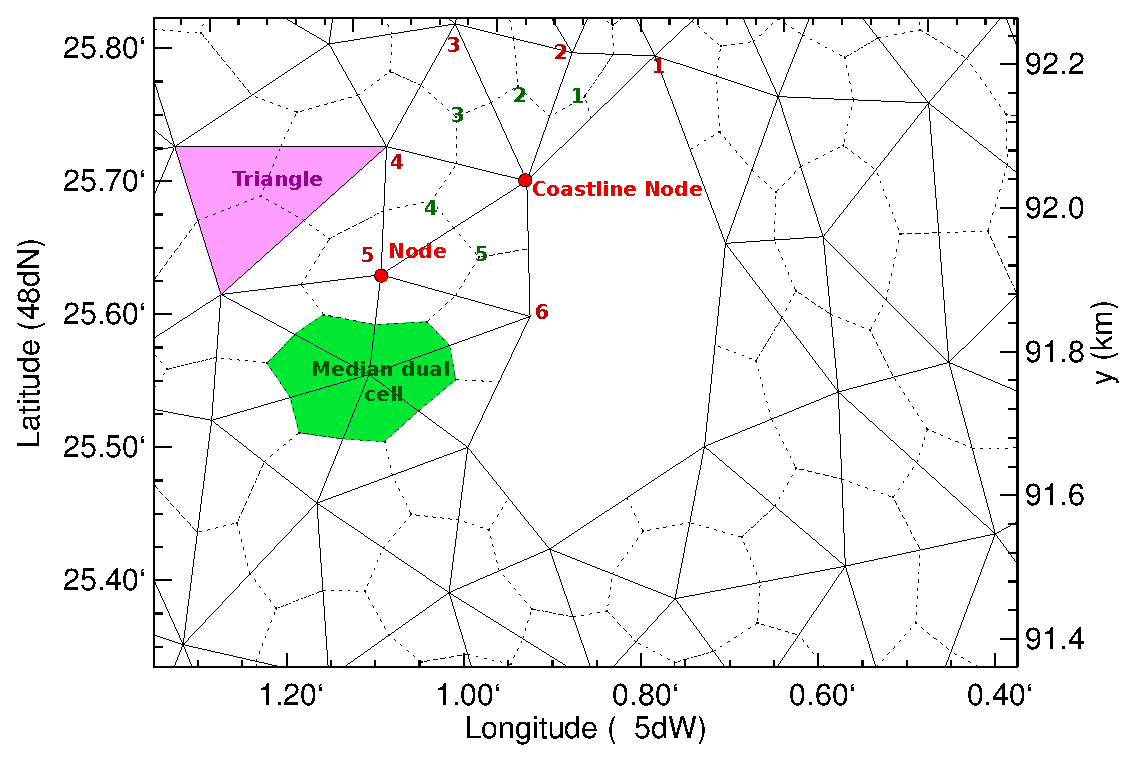
\epsfig{file=./num/grid_triangles.eps,angle=0,width=4.in}
\caption{Example of a region of a triangle-based mesh, with in this case the
 small Island of Bannec, France. If the depth is greater than the minimum
depth, the nodes of the shoreline are active. These are characterized by a
larger number of neighbor nodes (6 in the example chosen) than neighbor
triangles (5 in the same example).}
\label{fig:triangles} \botline
\end{center}
\end{figure}

